
\documentclass[12pt]{article}

\usepackage{physor2016}

\usepackage{amsmath}
\usepackage{bm}

\newcommand{\ve}[1]{\ensuremath{\mathbf{#1}}}
\newcommand{\Macro}{\ensuremath{\Sigma}}
\newcommand{\vOmega}{\ensuremath{\hat{\Omega}}}
\newcommand{\omvec}{\ensuremath{\hat{\Omega}}}
\newcommand{\rvec}{\ensuremath{\vec{r}}}
\newcommand{\vecr}{\ensuremath{\vec{r}}}

\usepackage{graphicx}
\usepackage{tikz}
\usepgflibrary{shapes.geometric}

\usepackage{booktabs}

\usepackage{siunitx}
%------------------------------------------------------------------------------

%------------------------------------------------------------------------------
% Define title. Use all CAPITALS.
%------------------------------------------------------------------------------
\title{AN ANGLE-INFORMED HYBRID METHOD FOR DEEP-PENETRATION RADIATION TRANSPORT APPLIED TO CADIS AND FW-CADIS}
%
% ...and authors
%
\author{ 
  \textbf{Madicken Munk and R.~N.~Slaybaugh} \\
  Department of Nuclear Engineering, University of California, Berkeley \\
  3115B Etcheverry Hall, Berkeley, CA 94720, USA\\
  \href{mailto:madicken@berkeley.edu}{madicken@berkeley.edu}\\
  \href{mailto:slaybaugh@berkeley.edu}{slaybaugh@berkeley.edu}\\
  \\
  \textbf{Tara M.~Pandya, Seth R.~Johnson, and T.~M.~Evans}\\
  Radiation Transport Group\\
  Oak Ridge National Laboratory, P.O.\ Box 2008, Oak Ridge, TN 37831, USA\\
  \href{mailto:pandyatm@ornl.gov}{pandyatm@ornl.gov}\\
  \href{mailto:johnsonsr@ornl.gov}{johnsonsr@ornl.gov}\\
  \href{mailto:evanstm@ornl.gov}{evanstm@ornl.gov}
  }
  
%------------------------------------------------------------------------------
\renewcommand{\shortauthor}      % Author's names here
           {M.\ Munk~et~al.}  
\renewcommand{\shorttitle}       % Short title here
           {Angle-Informed CADIS and FW-CADIS}  

%------------------------------------------------------------------------------
% Setup PDF info. This sets several values which are listed as the "properties"
% of the PDF file.
%------------------------------------------------------------------------------
\hypersetup{
  pdftitle=\shorttitle,
  pdfauthor=\shortauthor
}


\begin{document}

%\doublespacing

%\linenumbers

%------------------------------------------------------------------------------
% Make the titlepage and set the pagestyle to fancy throughout
%------------------------------------------------------------------------------
\maketitle

\begin{abstract}
This is our abstract
\end{abstract}

\keywords{Hybrid Methods, CADIS, FW-CADIS, Angular Biasing}

%------------------------------------------------------------------------------
%
%------------------------------------------------------------------------------
\section{INTRODUCTION}
\label{sect::intro}

Efficiently modeling radiation transport in deep penetration shielding problems is essential to the safe operation of many types of nuclear facilities as well as the development of monitoring and detection systems. We would like to be able to perform such calculations with Monte Carlo (MC) methods, but it can be quite challenging to obtain acceptable statistical uncertainties in the computed tallies. Thus, many variance reduction (VR) strategies, some of which we will discuss, have been developed to facilitate accurate calculations in reasonable times. 

Problems that exhibit a strong degree of angular anisotropy in particle flux, however, tend to be even more challenging for effective VR.
Many existing VR methods do not include angular information in their techniques, and therefore do not work well for these problems.  
Some VR methods do include angular information, but in general these methods have challenges in breadth of applicability or ease of use that make them inadequate as broad tools, or are too costly to use reliably in practice.

With the goal of filling some of these gaps, we have developed a new method that builds on the Consistent Adjoint Driven Importance Sampling (CADIS) and Forward Weighted-CADIS (FW-CADIS) methods~\cite{wagner_forward-weighted_2007} to tackle fixed-source problems that exhibit a high degree of angular anisotropy. 
This method builds on existing software infrastructure in a way that facilitates easy adoption.
CADIS and FW-CADIS, which we will jointly refer to FW/CADIS, use scalar flux estimates from a deterministic calcualtion to create VR parameters for use in MC.
Our new method uses a forward-weighted adjoint scalar flux based on a normalized contributon flux instead of a standard scalar flux.
This new integration scheme includes angular information in order to improve MC performance for problems with anisotropic particle fluxes.

We have implemented this method and tested it in two optically-thick source-detector labyrinth demonstration problems. 
These demonstration problems have characteristics that are particularly challenging for existing methods and provide an opportunity to start investigating differences between this new method and CADIS.
As such, we compare an analog calculation, a standard CADIS calculation, and a new angular CADIS calculation, henceforth referred to as CADIS-$\Omega$ (and FW/CADIS-$\Omega$ for both methods jointly). Initial results for these two geometries shows that for problems with strongly anisotropic behavior, CADIS-$\Omega$ outperforms traditional CADIS.

In this paper, we begin with a brief background (Section~\ref{sect::second}) of important concepts relating to variance reduction and existing hybrid methods for deep-penetration radiation transport.
We then provide the context of existing methods in Section~\ref{sect::past}. 
Section~\ref{sect::methodology} describes the mathematical foundation of our proposed method (Section~\ref{subsect::theory}) and the software that we used to implement it (Section~\ref{subsect::implementation}). 
The results and accompanying discussion are described in Section~\ref{sect::results}. Following this, Section~\ref{sect::future} presents our future test plans and details how this plan will map out the application space beyond this single demonstration test. 
We conclude in Section~\ref{sect::conclusion}. 


%------------------------------------------------------------------------------
%
%------------------------------------------------------------------------------
\section{BACKGROUND}
\label{sect::second}

This section provides the equations we are solving as well as background concepts that are used in many VR methods and ideas needed for our method in particular. 
Many modern radiation transport codes offer variance reduction capabilities that employ an importance map\textemdash a measure of how important a particular particle in a Monte Carlo simulation is to the tally being computed\textemdash which is related to the adjoint form of the transport equation. 
%Using this importance information, the Monte Carlo code can spend more time on important particles and less time on unimportant particles. This reduces the statistical variance in the final tally result for a given amount of computational time, providing better results in less time. 
Our method's algorithm also incorporates a weighted variant of the contributon flux, which 
Our new method also uses contributons, which (words about contributons) ~\cite{williams_contributorn_1992}. 

%Write forward and adjoint importance equation and define terms\\
The steady state, fixed-source forms of the forward and adjoint transport equation are
\begin{align*}
\bigl[\hat{\Omega} \cdot \nabla + \Macro_t(\vec{r}, E)\bigr] \psi(\vec{r}, \hat{\Omega}, E)  =  \int_0^{\infty} dE' &\int_{4\pi} d\hat{\Omega'} \:\Macro_{s}(\vec{r}, E' \to E, \hat{\Omega'} \cdot \hat{\Omega}) \psi(\vec{r}, \hat{\Omega'}, E') + q(\vec{r}, \vOmega, E)\\
%
\bigl[-\vOmega \cdot \nabla + \Sigma_t(\rvec, E)\bigr] \psi^{\dagger}(\vec{r}, \vOmega, E) = \int_0^{\infty} dE' &\int_{4\pi} d\vOmega' \: \Sigma_s(\rvec, E \rightarrow E', \vOmega \cdot \vOmega') \psi^{\dagger}(\rvec, \vOmega', E') \\
&+ q^{\dagger}(\vec{r}, \vOmega, E)\:,
\end{align*}
respectively, where $\psi(\vec{r}, \hat{\Omega}, E)$ is the angular neutron flux, $\Sigma_t$ is the total macroscopic cross section, $\Sigma_s$ is the double-differential scattering cross section, $q$ is a fixed source, and superscript $\dagger$ indicates adjoint quantities. 

% explain Adjoint = Importance; point out this is a concept frequently used in variance reduction (some starting language?)\\
The angular adjoint flux can represent a map of how every part of phase space will influence the answer we are looking for.
That is $\psi$ represents how the source particles go forward and affect the rest of the problem space; $\psi^{\dagger}$ represents how the particles from a source come into the solution space and affect the answer. 

explain Contributon = Response; give any context about use of contributons \\

\section{PAST WORK}
\label{sect::past}
Highlight the CADIS method \\
Highlight the FW-CADIS method \\
Talk about what problems CADIS and FW-CADIS succeed in, then talk about where they fall short. \\

Examples of variance reduction using importance maps include the weight window generator/weight window map (WWG) capability in the MCNP Monte Carlo code~\cite{brown_mcnp_2002}, and the FW/CADIS methods. Target weights in weight window maps are the inverse of the importance values for a given point in phase space.

For problems with very strong anisotropies in the particle flux, such as the streaming found near the air vents of an individual cask or in between casks stored in an array pattern, the importance map and biased source developed using the space/energy treatment above may not represent the real importance well enough to sufficiently accelerate the Monte Carlo calculation. Notice that the angular dependence of the importance function is not retained, because otherwise the map would be very large (tens or hundreds of GB) and more costly and complex to use in the Monte Carlo simulation. 

The drawback of this simplification is that, within a given space/energy cell, the map provides the average importance of a particle moving in any direction through the cell—excluding information about how particles move toward the objective. Consider the simple labyrinth example shown in Figure 1. For a source at the left entrance, the dose rate inside and outside of the labyrinth ranges over 12 orders of magnitude. Analog Monte Carlo would have to sample trillions of particles to get a few to the lowest dose regions. The space/energy treatment used in FW-CADIS makes this problem tractable but challenging. For particles near the turns in the labyrinth, the importance of the particles to the exit of the labyrinth vary greatly if they are coming out of a wall pointed toward the exit versus heading into a wall and away from the exit. This distinction is not captured by current hybrid methods. Including angular information in the importance map should significantly improve the Monte Carlo run time. 

Introduce angle-informed and angle-biased methods. \\
Higlight AVATAR + shortcomings \\
Highlight Turner \& Larsen's method + shortcomings\\

To do fast, accurate transport for used fuel monitoring, what is needed is an importance map generated quickly using deterministic methods that captures the impact of angle in the importance information. A variety of strategies for accomplishing this goal have been tried over the years. One such method is the Local Importance Function Transform (LIFT) method [10], which is derived from the zero-variance method and  uses an approximation of the adjoint flux that is piecewise continuous in angle. LIFT only captures linearly anisotropic scattering, which is not enough for our needs and is somewhat difficult to use [11].

More recently, an attempt by Peplow et al. [12] to solve this problem used the maximum entropy distribution [13] to approximate the angular adjoint flux, , and showed improvement in some problems but very little in others. In that work, the angular component of the adjoint flux was approximated as separable and symmetric about the average adjoint current direction. We will refer to this method as simple angular CADIS. Two versions were implemented, one with (limited) directional source biasing and one without. The method without source biasing is effectively the method used by the AVATAR [14] code on a Cartesian mesh and on a tet-mesh in a code by Evans and Wareing [13]. 

In Peplow et al.’s work, the improvement using simple angular CADIS over standard CADIS ranged from a factor of 0.09 to 3.3 over a collection of eight test problems, many of which have characteristics similar to used fuel cask monitoring systems. In all cases, CADIS and simple angular CADIS outperformed analog Monte Carlo. Peplow et al.’s study demonstrated that in many cases in which anisotropies are important, including angular information will improve calculation efficiency. However, these results also showed that the simple angular CADIS implementation is not accurate enough to provide the improvement necessary to be able to efficiently execute the used fuel cask calculations we would like to perform to improve facility monitoring design and operation. We therefore need to develop a better method for capturing the angular information.  
	


Conclude section with discussion of what is missing from CADIS/FW-CADIS/Angle Methods to motivate new method. \\

%------------------------------------------------------------------------------
%
%------------------------------------------------------------------------------
\section{METHODOLOGY}
\label{sect::methodology}

Introduce section with goal of our method. \\

%------------------------------------------------------------------------------
%
%------------------------------------------------------------------------------
\subsection{Theory}
\label{subsect::theory}

Show our method equation. \\


\begin{equation} 
\label{eq:angularhybrid}
\phi^{+}(\vec{r},E) = \frac{\int \psi(\vec {r} ,E,\hat{\Omega})\psi^+(\vec {r} ,E,\hat{\Omega})d\hat\Omega }{\int\psi(\vec {r} ,E,\hat{\Omega})d\hat\Omega}
\end{equation}


Discuss how this relates to the concept of importance with the adjoint. \\
Discuss how this relates to contributon response. \\
Say physically how this helps us track in problems with strong anisotropy. \\
Highlight how this is different from past methods.

%------------------------------------------------------------------------------
%
%------------------------------------------------------------------------------

\subsection{Implementation}
\label{subsect::implementation}

We implemented the new method through the AutomateD VAriaNce reducTion Generator\\ (ADVANTG)~\cite{wagner_automated_2002, mosher_new_2010} software developed at ORNL. 
ADVANTG automates the generation of the importance map and biased source distribution created using either the CADIS or FW-CADIS methods for use in MCNP5~\cite{brown_mcnp_2002}. 
An input file in MCNP syntax is provided by the user in addition to some instructions for running ADVANTG. 
ADVANTG uses this information to generate input file(s) and exectues the discrete ordinates solver Denovo~\cite{evans_denovo:_2010} in adjoint or forward and adjoint mode, as appropriate.
The deterministic calculations can be performed using multiple cores and/or processors (e.g., on multi-core desktop systems and clusters). 
ADVANTG takes Denovo's output, executes the CADIS or FW-CADIS methods, and the final variance reduction parameters are output in a format that can be used with unmodified versions of MCNP. 
The primary objective of the development of ADVANTG has been to reduce both the user effort and the computational time required to obtain accurate and precise tally estimates
across a broad range of challenging transport application areas.

We chose to use ADVANTG for several key reasons. 
The most important is that the implementation is nearly invisible to the user and therefore their experience of using this method will be nearly identical to using CADIS or FW-CADIS.
That is, the user simply adds an additional instruction asking to use the angle informed method and the interface does not change otherwise.
This facilitates easy adoption.
Further, only one MCNP input file is required to compare the new method to FW/CADIS.
Finally, it was simpler to implement the new method through ADVANTG than starting separately as we could take advantage of so much existing infrastructure in the coupling.

The major modifications required to implement this method were to Denovo. 
The angular flux is typically not stored or written as the desired output is typically the scalar flux.
The new method, however, requires the angular flux to create the scalar flux, and therefore Denovo was modified to store and write the angular flux.
A new function was also added that takes the forward and adjoint fluxes and performs the integration indicated in eqn.~\eqref{eq::angularhybrid}. 
This set of scalar fluxes is then written the same way as any scalar flux output from Denovo.

The benefit the bulk of the implementation being in Denovo is several fold. 
From the standpoint of ADVANTG, there are very few differences between the new method and FW/CADIS and therefore implementation is straightforward.
Further, anyone who finds a use for a scalar flux created as in eqn.~\eqref{eq::angularhybrid} will now be able  access it.
Finally, it might be useful to have access to the full angular flux. 
Examining the angular flux for a problem could have research or pedagogical implications, and some other variance reduction method that uses the angular flux explicitly could be more easily developed in the future.

%------------------------------------------------------------------------------
%
%------------------------------------------------------------------------------
\section{RESULTS AND DISCUSSION} 
\label{sect::results}

To begin to characterize the performance of CADIS-$\Omega$ we chose two labyrinth source-detector test problems.
Such labyrinth problems contain some angle dependence that is not well captured by standard CADIS~\cite{Peplow-ORNL}. 
The motivation for these initial tests is to investigate the differences between CADIS and CADIS-$\Omega$.
We will therefore examine the adjoint scalar fluxes, which are effectively the importance maps, and the Monte Carlo figures of merit (FOMs) produced by each method, where 
\[\text{FOM} = \frac{\text{calculation time}}{(\text{average relative error})^2}\:. \]
% State what RE you used in computing the FOMs.
We also performed an analog calculation with each geometry, comparing  the tally result, the relative uncertainty, and the FOM of the response tally (f4) for all three methods.
All methods used NUMBER OF PARTICLES. 
The CADIS methods used LIST SN PARAMETERS (SN, PN, \# MESH CELLS, SPATIAL SOLVER).

Figure~\ref{fig::fwdflux} shows each geometry overlaid on a forward deterministic flux map. 
Labyrinth I (top) contains a Li-doped polyethylene shield, and Labyrinth II (bottom) contains a concrete shield. 
Each problem has reflective boundary conditions,
% If we get to rerun these at some point I would create actual walls or use black boundary conditions.
 a 10MeV, isotropic point source at (-75, 0, 0), and a NaI detector on the other side of the shield at (LOCATION) and (LOCATION), respectively. 
CADIS and CADIS-$\Omega$ were set to optimize the response in the NaI detector. 
\begin{figure}
  \begin{center}
    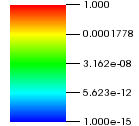
\includegraphics[width=0.10\textwidth]{./images/scale.png}
    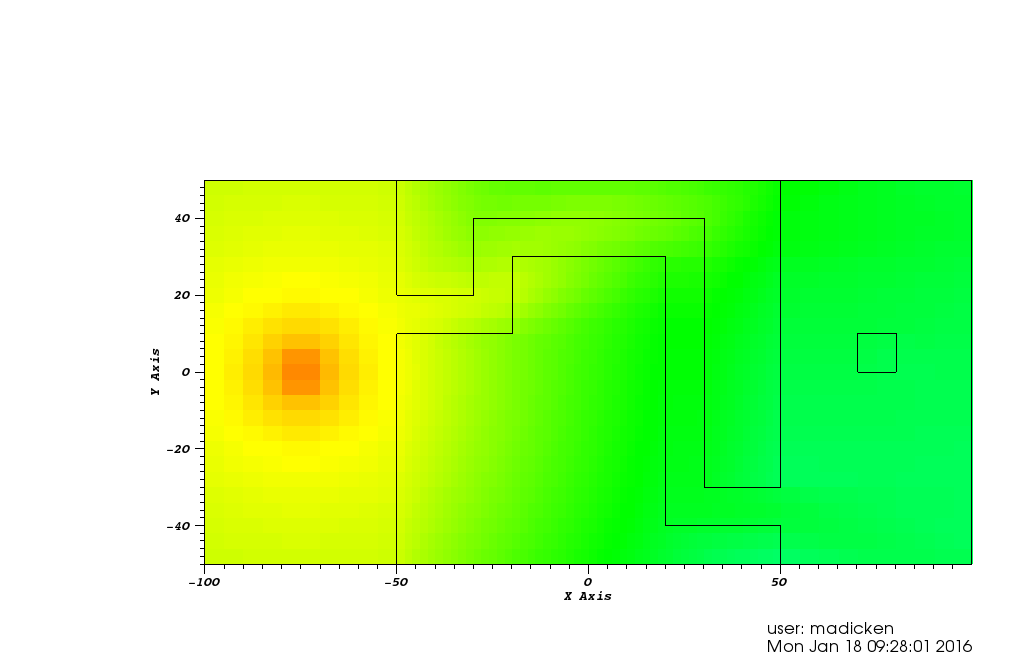
\includegraphics[width=0.80\textwidth]{./images/forward_flux.png}
    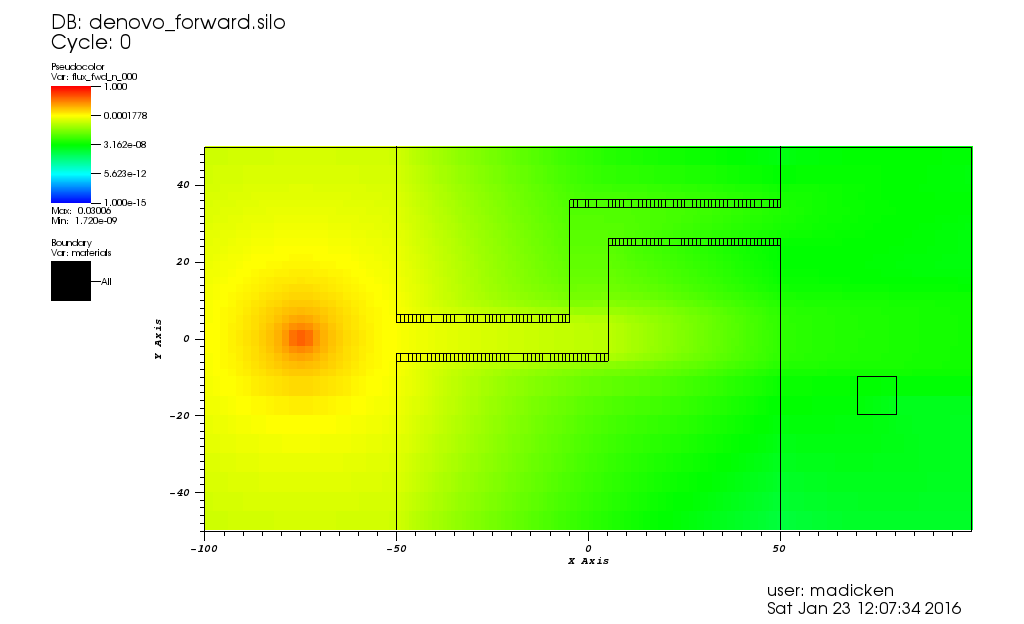
\includegraphics[width=0.80\textwidth]{./images/maze2_forward_group00_adjusted.png}
    \caption[]{\label{fig::fwdflux}Forward deterministic flux generated by Denovo for Labyrinth problems I (top) and II (bottom). Dimensions are in cm; the plots use the same color scale.}
  \end{center}
\end{figure}
% the axes and labels are really hard to read 

\begin{figure}
  \begin{center}
    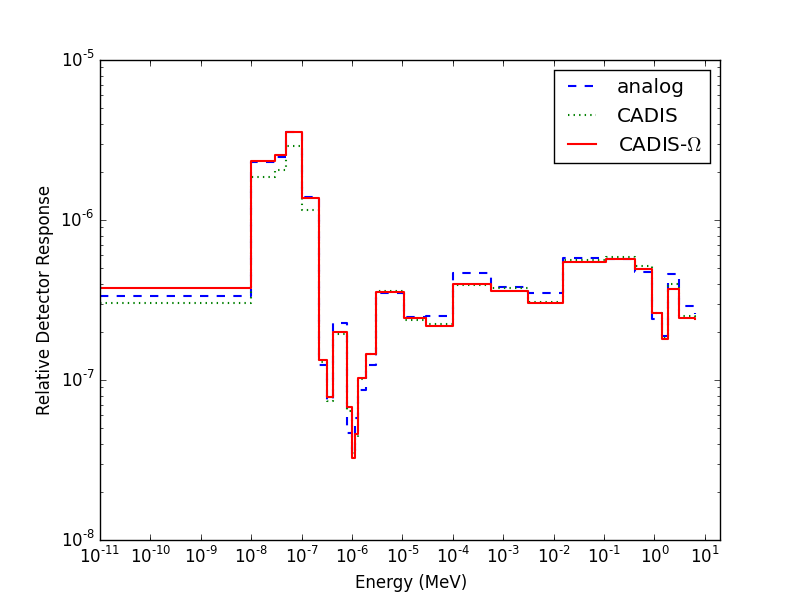
\includegraphics[width=0.49\textwidth]{./images/maze2_spectra.png}
    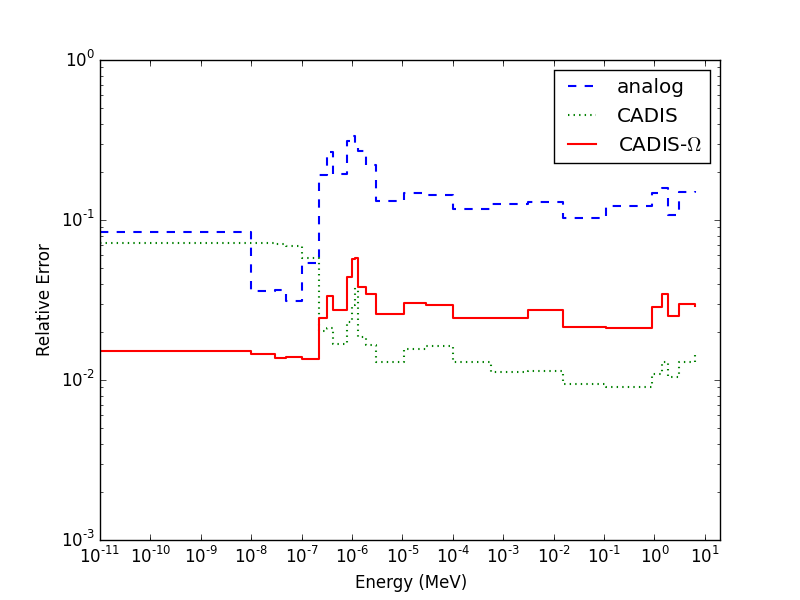
\includegraphics[width=0.49\textwidth]{./images/maze2_RE.png}
    \caption[]{\label{fig::tallyresponse} Responses (left) and relative uncertainties (right) in NaI detector tally for the Labyrinth II problem. }
  \end{center}
\end{figure}
% Axes aren't great, hard to read the CADIS line
% These need error bars if possible, otherwise it is very difficult to compare

The tally responses and relative uncertainties for the NaI detector in Labyrinth II are shown in Figure \ref{fig::tallyresponse} for all methods. 
The responses are equivalent to within one standard deviation. 
% Is this true? Plots need error bars so we can tell.
The CADIS method took LIST TIME HERE and CADIS-$\Omega$ took LIST TIME HERE on NUMBER OF CORES on PLATFORM, resulting in FOMs of 9 and 94, respectively.
CADIS-$\Omega$ has a lower relative error than CADIS for lower energy bins, but a higher relative error for higher energy bins. 
To investigate the reason that CADIS-$\Omega$ has higher relative error in some energies, we compared the adjoint fluxes generated by CADIS and CADIS-$\Omega$ in a higher energy group, group 26 (ENERGY RANGE) and seen in Figure~\ref{fig::adjoint_fluxes_group26}, and a lower energy group, group 11 (ENERGY RANGE), and seen in Figure~\ref{fig::adjoint_fluxes_group11}.
Note that in these figures the color scales are not the same so that the relative behavior of the flux within a method can be compared between the methods. 

\begin{figure}
  \begin{center}
    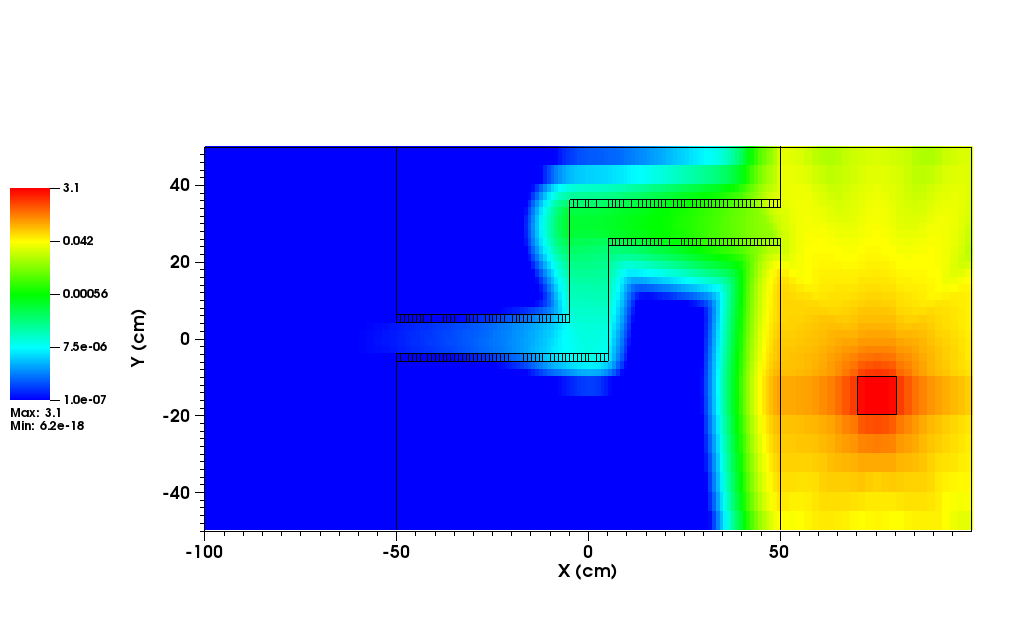
\includegraphics[width=0.80\textwidth]{./images/maze2_adjoint_group26_adjusted.png}
    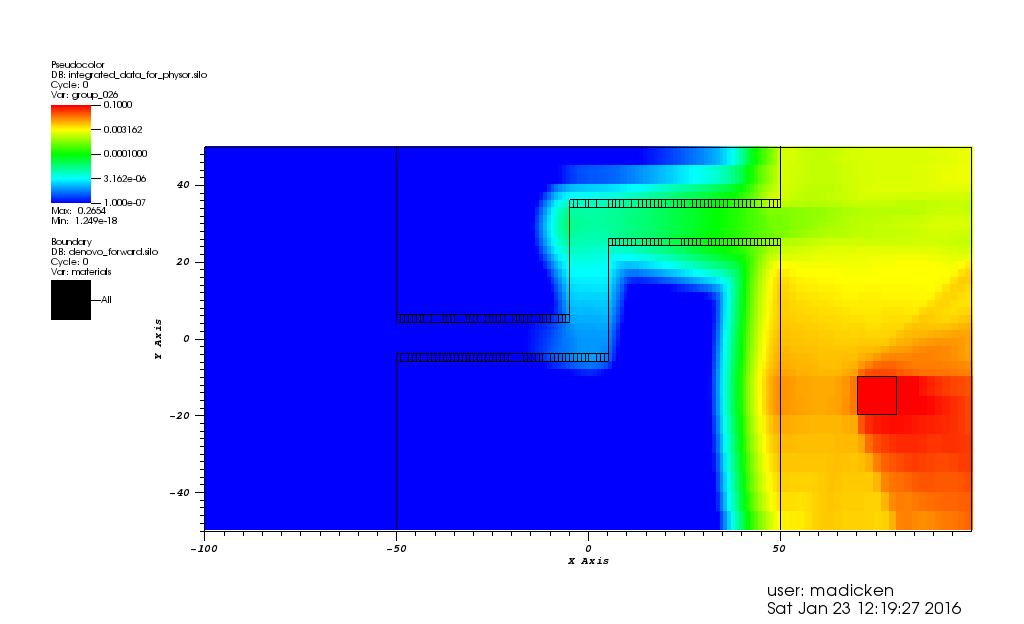
\includegraphics[width=0.80\textwidth]{./images/maze2_myflux_group26_adjusted.png}
    \caption[]{\label{fig::adjoint_fluxes_group26}\textit{Group 26} adjoint flux generated by standard Denovo (top) and CADIS-$\Omega$ method (bottom) for Labyrinth II geometry.}
  \end{center}
\end{figure}

\begin{figure}
  \begin{center}
    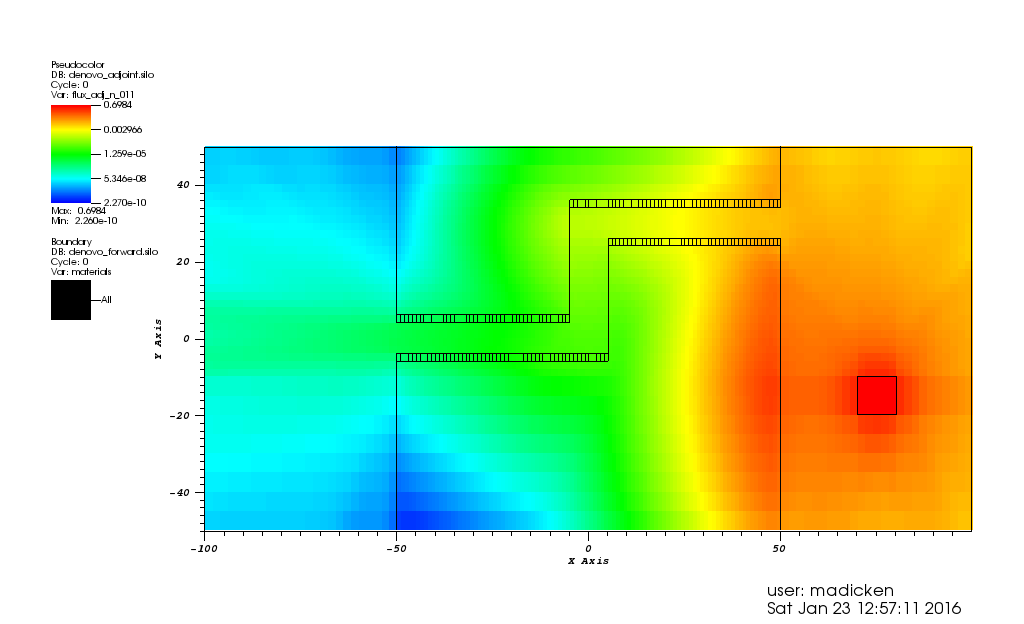
\includegraphics[width=0.80\textwidth]{./images/maze2_adjoint_group11_adjusted.png}
    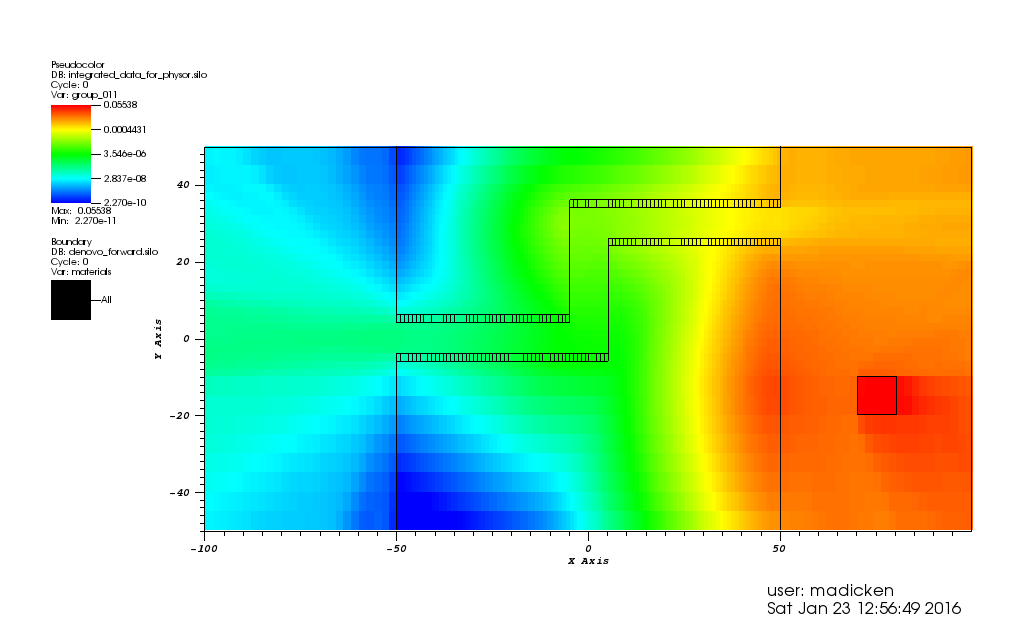
\includegraphics[width=0.80\textwidth]{./images/maze2_myflux_group11_adjusted.png}
    \caption[]{\label{fig::adjoint_fluxes_group11}\textit{Group 11} adjoint flux generated by standard Denovo (top) and CADIS-$\Omega$ method (bottom) for Labyrinth II geometry.}
  \end{center}
\end{figure}

In group 26, CADIS-$\Omega$ creates an adjoint flux in which the majority of the group 26 neutrons that contribute to the detector response are reflected off of the back and bottom walls, while the standard adjoint indicates fairly symmetric contribution. 
This illustrates that CADIS-$\Omega$ captures angular information differently than CADIS. 
We expect the shape of the CADIS map given the non-inclusion of angular information. 
The CADIS-$\Omega$ map seems to STATEMENT ABOUT WHAT WE THINK ABOUT THIS BEHAVIOR.

This asymmetric effect in the CADIS-$\Omega$ case is not as prominent in group 11. 
This is likely because of the differences in the survival probability of a group 11 neutron compared to a group 26 neutron hitting the concrete wall. 
That is, the group 11 neutrons are far more likely to return to the detector after hitting the concrete wall than group 26, 
%is that true?
 resulting in a more locally-isotropic flux near the detector. 
As a result, the group 11 CADIS-$\Omega$ adjoint fluxes more closely match the adjoint fluxes generated by CADIS. 
 
MAKE SOME STATEMENTS ABOUT WHY THAT IMPACTS RELATIVE ERROR AND THE FOMs.\\
Discuss differences and meaning of differences of results and parameter maps \\
Discuss implications of these differences for solving other problems more generally

%As mentioned in Section \ref{subsect::theory}, the strength of this method is that it biases particles in the direction that they will actually be moving, rather than just towards the adjoint source.
%By adjusting the scales of the adjoint flux generated by CADIS and CADIS-$\Omega$, one can compare the biasing parameters for each problem. Figure \ref{fig::adjoint_fluxes_group26} adjusts the scales for Labyrinth II in group 26, and Figure \ref{fig::adjoint_fluxes_group11} do so for group 11. It is quite noticeable that the majority of particles contributing to the NaI detector response in group 26 are reflected off of the right- and bottom- boundaries. This effect is also visible in figure \ref{fig::adjoint_fluxes_group11}, but is not as strong.  
% This paragraph isn't really needed.

 \begin{table}
  \centering
  \caption{\label{tab:FOMLabI}FOMs for Labyrinth Problems}
  \begin{tabular}{l|cc|cc}
    \toprule
        & \multicolumn{2}{c}{Labyrinth I} & \multicolumn{2}{c}{Labyrinth II}  \\
    \hline
        & FOM$_{MC}$ & FOM$_{adjusted}$ & FOM$_{MC}$ & FOM$_{adjusted}$ \\
    \hline
    Analog           & 26    &  26  & 538 & 538 \\ 
    CADIS            & 1419  &  799 & 31  &  9  \\
    CADIS-$\Omega$   & 1282  &  248 & 354 & 94  \\  
	\bottomrule
  \end{tabular}
\end{table}

% Note: these FOMs don't really make sense to me. Why is the analog problem so good in Labyrinth II but not in I? Is the material choice of the shield really that significant? That's the only thing I can come up with to explain this. I guess 100cm of concrete is possible for neutrons to make it through, but the poly has such a strong absorber in the Li that it makes it more difficult to penetrate. 

Table \ref{tab:FOMLabI} reports FOMs for both problems and all methods using the Monte Carlo simulation alone (designated MC), as well as an adjusted FOM that incorporates the runtimes for deterministic transport (designated adjusted). 
Even when incorporating the deterministic transport time, the biased calculations perform significantly better than the analog problem for Labyrinth I but not Labyrinth II. 
We believe that this is due to the high absorption in the shield in Labyrinth I compared to more scattering in Labyrinth II. 
% This doesn't make any sense...
For a simple problem with the refined angular and spatial discretizations we chose, the deterministic calculation times were comparatively significant.
Because CADIS-$\Omega$ uses two deterministic transport calculations while CADIS uses one, incorporating the increased time for the calculation is necessary for a fair comparison.
It is worth noting that FW-CADIS-$\Omega$ and FW-CADIS would no longer have this discrepancy in deterministic calculation time.
 
MORE EXPLANATION AND DISCUSSION?

Table \ref{tab:FOMLabI} also shows that CADIS-$\Omega$ outperforms CADIS in Labyrinth II, and performs less well than CADIS in Labyrinth I. This is likely due to the large number of turns in Labyrinth I. 
% This would be an easier statement to make if they had the same materials...I guess I should have thought of that. We should probably say something about the materials. 
Any neutron that does make it through Labyrinth I is likely to have scattered several times, rendering the flux throughout the maze channels to be relatively isotropic and reducing the effect of the method. However, this effect is not as significant in Labyrinth II as it is in Labyrinth I, which is likely why CADIS-$\Omega$ outperforms CADIS in this problem. 

Overall the performance of CADIS-$\Omega$ compared to CADIS and analog MC is WORDS THAT MAKE A MINI SUMMARY. 
Based on both theory and the differences in the results between geometries, we expect that this method will perform well in problems with strong streaming paths and less well in problems with significant scattering effects. 
 


%------------------------------------------------------------------------------
%
%------------------------------------------------------------------------------
\section{FUTURE WORK} 
\label{sect::future}
 
Section \ref{sect::results} showed that CADIS-$\Omega$ can outperform CADIS in a problem with a strong degree of angular anisotropy in the flux. However, there are a number of physical means by which angular anisotropy in the flux might occur. To further characterize the performance of CADIS-$\Omega$ and FW-CADIS-$\Omega$ throughout all of these problems, we are planning to use a suite of test problems that should help quantify the performance of the method. The testing phase space identified in Table \ref{tab:testprobs} summarizes our testing plans. As noted in Section \ref{sect::results}, problems where the direction of particles is important to the importance of a cell are where we anticipate the strength to lie in CADIS-$\Omega$. These problems aim to address all of the physical means by which the flux could become strongly anisotropic, and some have shown to be difficult for traditional FW/CADIS~\citep{Peplow-ORNL}. 

 \begin{table}
  \centering
  \caption{Proposed Test Problem Coverage}
  \begin{tabular}{l|cccc}
    \toprule
    Problem Name & \multicolumn{4}{c}{Problem Coverage} \\
    \hline
     & Streaming Paths & High Scatter & Highly Heterog. & Beam Problem \\
    \hline
    Streaming Channel   & X & & & X \\ 
    Metal Plate         & X & X & X &  \\
    Labyrinth Variants  & X & X & X &  \\ 
    Spherical Boat      & X & & X & X \\  
    Kobayashi Benchmark & X & X &  &  \\   
	\bottomrule
  \end{tabular}
  \label{tab:testprobs}
\end{table}

After FW/CADIS-$\Omega$ has been fully characterized throughout the phase space identified in Table \ref{tab:testprobs}, it will be tested with large problems of interest. 
Specifically, we are interested in real problems that contain strong angular anisotropies that are difficult to solve, such as active interrogation problems, spent fuel cask storage (through air vents and between casks on ISFISIs), and facility calculations containing long gaps or streaming materials embedded in moderators. 
These large problem studies will be informed by the small problem studies and demonstrate the potential impact of this new method. 

%As with the simple problems performed in Section \ref{sect::results}, the results of FW/CADIS-$\Omega$ will be compared to traditional FW/CADIS. The FOM, the tally uncertainty distribution, and the tally results will be indicators of the success of the -$\Omega$ methods. 
% Unnecessary

%------------------------------------------------------------------------------
%
%------------------------------------------------------------------------------
\section{CONCLUSION} 
\label{sect::conclusion}

Recap what we told them (what problem we're trying to solve; about this method; how it's different than past methods)\\
Recap problem we solved and results\\
Strong punchline paragraph about potential impact based on theory and these results.

The testing phase of this project aims to (1) characterize the method's performance in a variety of problems that have anisotropies, and (2) compare how well the method performs compared to traditional CADIS and FW-CADIS.

%------------------------------------------------------------------------------
%
%------------------------------------------------------------------------------
\section*{ACKNOWLEDGMENTS}

This material is based on work supported by the Department of Energy under award number DE-NE0008286. This report was prepared as an account of work sponsored by an agency of the United States Government. Neither the United States Government nor any agency thereof, nor any of their employees, makes any warranty, express or implied, or assumes any legal liability or responsibility for the accuracy, completeness, or usefulness of any information, apparatus, product, or process disclosed, or represents that its use would not infringe privately owned rights. Reference herein to any specific commercial product, process, or service by trade name, trademark, manufacturer, or otherwise does not necessarily constitute or imply its endorsement, recommendation, or favoring by the United States Government or any agency thereof. The views and opinions of the authors expressed herein do not necessarily state or reflect those of the United States Government or any agency thereof.

\bibliographystyle{physor2016}
\bibliography{physor2016}

\appendix

\makeatletter
\def\@seccntformat#1{APPENDIX \csname the#1\endcsname.~}
\makeatother

%------------------------------------------------------------------------------
% If you need to make one (or more) appendix (appendices), place them here as
% sections
%------------------------------------------------------------------------------
\section{HOW TO MAKE APPENDICES}
\label{app::a}

This is a placeholder for my first appendix

\section{OTHER APPENDIX STUFF}
\label{app::b}

This is a placeholder for my second appendix

\end{document}

